This chapter provides procedures for setting up NetWorkSpaces
and Sleigh for MATLAB.  See the INSTALL and README files in the
NetWorkSpaces distribution for more information.

\section{Prerequisites}
NetWorkSpaces runs on Linux, Max OS X, Windows, and most Unix systems.
The MATLAB NWS API has no prerequisites, other than MATLAB 7.0 or later.
However, you must be running a NetWorkSpaces server on some network
accessible machine (which includes the local machine, of course).  The
server is a Python/Twisted application, and therefore requires Python
with Twisted installed.  NetWorkSpaces uses Twisted Core and Twisted
Web, and Twisted in turns requires Zope Interfaces, which comes bundled
with the Twisted installation.

To summarize:
\begin{itemize}
\item MATLAB 7.0 or later \url{http://www.mathworks.com}
\item Python 2.2 or later \url{http://www.python.org}
\item NetWorkSpaces server \url{http://nws-py.sourceforge.net}
\item Twisted Core 2.1 or later \url{http://twistedmatrix.com}
\item Twisted Web 0.5 or later
\item Zope Interfaces (as distributed with Twisted)
\end{itemize}

Note on Windows, NetWorkSpaces has an ``all-in-one'' installer that will
install everything that you need to run the server, MATLAB~NWS~API,
Python~NWS~API, and R~NWS~API, so if you choose to use that, you don't
have to be aware of these software requirements.

\section{NetWorkSpaces Server}
\subsection{Starting the Server}
There are several ways to start a NetWorkSpaces server.
If you install NetWorkSpaces on Windows with the ``all-in-one''
installer, than the server is already running as the
``NwsService''.  You can check on it's status, start, and stop it using
the standard Windows tools.

\begin{itemize}
\item {twistd command (as daemon):}
\begin{verbatim}
% twistd -y /etc/nws.tac
\end{verbatim}

Note: nws.tac is installed in different directories, depending on
the platform and the type of installation (root versus non-root).
For root installation, nws.tac is located in \texttt{/etc} on UNIX,
and in the PYTHON24 or PYTHON25 directory on Windows. 
\item {nws script (UNIX only):} \\
The nws script is intended to be an init script, but it can be
used manually, as follows:
\begin{verbatim}
% nws start
\end{verbatim}
\item {NwsService (Windows only):} \\
If you didn't install NetWorkSpaces using the ``all-in-one'' installer, the
procedure installing and running the service is:
\begin{enumerate}
\item Open up a command prompt
\item Install NwsService by executing NwsService.py, which is located in Python's scripts directory
\begin{verbatim}
C:\python25\scripts> python NwsService.py install
\end{verbatim}
\item Start NwsService
\begin{verbatim}
C:\> sc start nwsservice
\end{verbatim}
\end{enumerate}
\end{itemize}

\subsection{Stopping the Server}
There are several ways to stop the NetWorkSpaces server:
\begin{itemize}
\item {If started via twistd:} \\
Go the directory where twistd was executed and type:
\begin{verbatim}
% kill `cat twistd.pid`
\end{verbatim}
\item {If started via nws script:}
\begin{verbatim}
% nws stop
\end{verbatim}
\item {If started via NwsService:}
\begin{verbatim}
C:\> sc stop nwsservice
\end{verbatim}
\end{itemize}

\section{NetWorkSpaces Client}
\subsection{Installing the Client}
To install NetWorkSpaces on Linux platforms:

\begin{itemize}
\item untar the nws package: tar xzvf nws\_matlab\_$<$version$>$.tar.gz
\end{itemize}

To install NetWorkSpaces on Windows:

\begin{itemize}
\item unzip the nws package.
\end{itemize}

\subsection{Setting MATLABPATH}
Make sure MATLABPATH contains the location of installed NetWorkSpaces.
If MATLABPATH is not setup correctly, then MATLAB will not know anything about NetWorkSpaces and Sleigh.

For example, on Linux, if NetWorkSpaces is installed in
/usr/local/nws\_matlab\_1.3, then add the following statement to your
shell startup script:

\begin{verbatim}
export MATLABPATH=/usr/local/nws_matlab_1.3:$MATLABPATH
\end{verbatim}

For Windows, open up a MATLAB session, and follow these steps:

\begin{enumerate}
\item Click the File Menu.
\item Click `Set Path'.
\item Click the `Add Folder' button.
\item Select the location of installed NetWorkSpaces.
\item Click `Save'.
\end{enumerate}

\subsection{Start NetWorkSpaces Client}
Once you've got a NetWorkSpace server up and running, you're ready to use NetWorkSpaces.

\begin{enumerate}
\item Start up a MATLAB session.
\item Type the following:
\begin{samepage}
\begin{verbatim}
>> ws = netWorkSpace('matlab space');
>> store(ws, 'x', 1);
\end{verbatim}
\end{samepage}
\end{enumerate}

This step creates a workspace named `matlab space' and stores a variable
\texttt{x} with value 1 to the workspace.

If you've encountered an error importing the NetWorkSpace class, it's likely
that you didn't set up MATLABPATH correctly.

You can also view what's in the workspace using a web interface.  To do this,
you point your browser to http://\textit{nwsserver}:8766, where
\textit{nwsserver} is the machine where the NetWorkSpaces server resides.
It should look something like this:

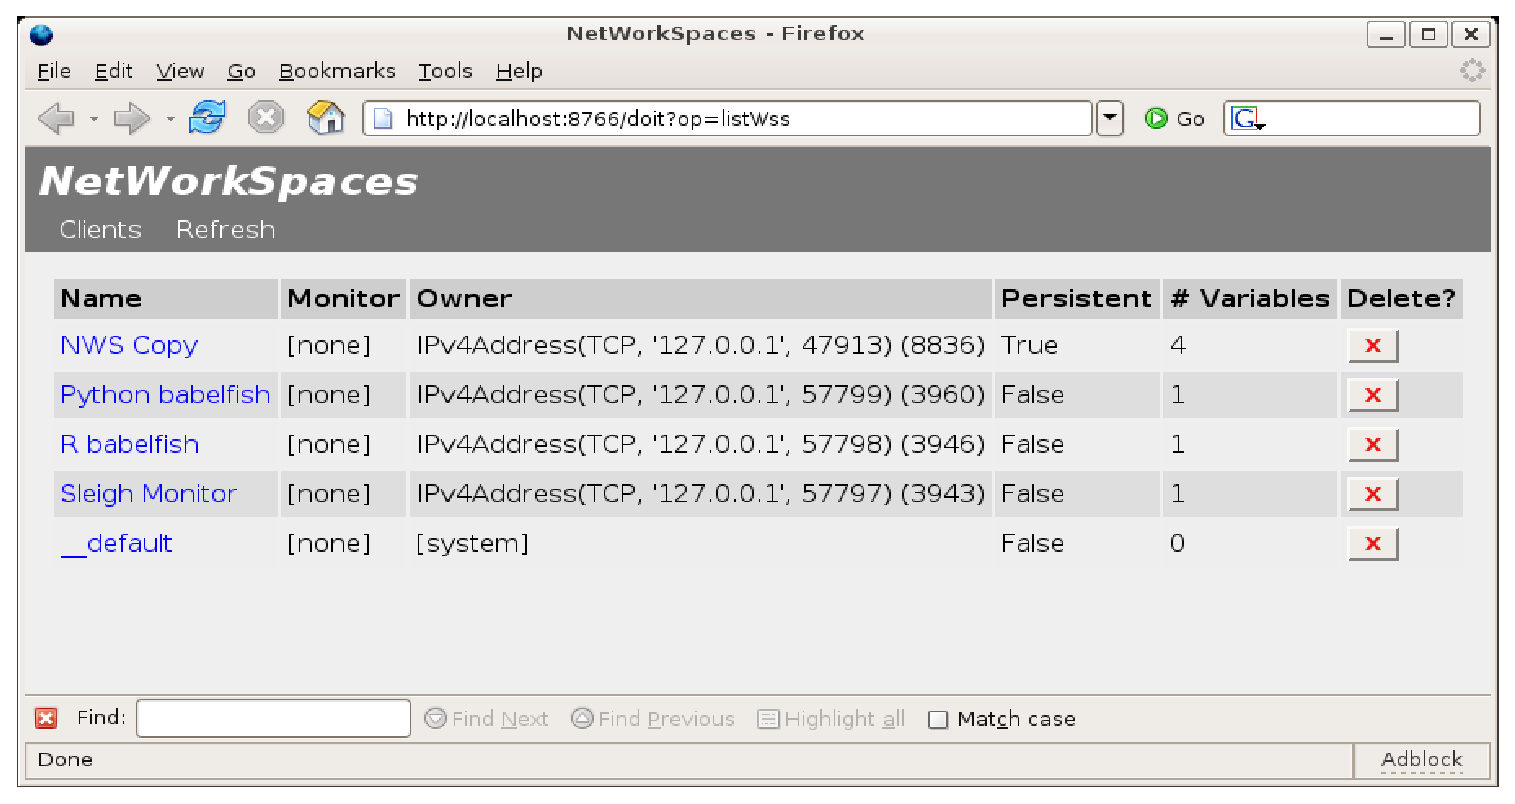
\includegraphics[width=5.95in]{webinterface.eps}

In order to examine the values that you've created from MATLAB in a
workspace using the server's web interface, you'll usually need to have
the MATLAB babelfish running.  The babelfish translates values into a
human readable format so they can be displayed in a web browser.  If a
value is a string, then the web interface simply displays the contents
of the string, without any help from the babelfish, but if the value is
any other type of MATLAB object, it needs help the help of the MATLAB
babelfish.

To run the babelfish, start another MATLAB session on the same machine
that is running the NWS server, and type the following command:

\begin{verbatim}
>> babelfish
\end{verbatim}

Note: this function will not return until you exit your MATLAB session.

For more examples on using NetWorkSpaces, see the Tutorials chapter.

\section{Starting Sleigh}
Sleigh is a MATLAB class, built on top of NetWorkSpaces, that makes it
very easy to write simple parallel programs.  Sleigh has a concept of one
master and multiple workers.  The master sends tasks to the workers who may or
may not be on the same machine as the master.  To enable the master to
communicate with workers, Sleigh supports several mechanisms to launch workers
which execute tasks.

\subsection{Local Launch Mechanism}
The local launch mechanism is the default launch option, and is used for
starting workers on the local machine.  By default, local launch starts
three workers, but you can specify the number of workers to launch by
setting the \texttt{workerCount} variable in the sOpts argument to the
sleigh constructor.  Local launch is useful for developing NetWorkSpace
programs, but it's also the best choice when running on a
multicore/multiprocessor computer.

Here's how to create a Sleigh object:

\begin{samepage}
\begin{verbatim}
>> s = sleigh()
\end{verbatim}
\end{samepage}

This is equivalent to:

\begin{samepage}
\begin{verbatim}
>> sOpts.launch = 'local';
>> s = sleigh(sOpts);
\end{verbatim}
\end{samepage}

\subsection{SSH Launch Mechanism}
To start up workers on machines other than your local computer, you need
to use a remote execution mechanism.  SSH is the most common method on
Unix-like systems.  To use SSH with NetWorkSpaces, set the launch
variable to the \texttt{sshcmd} function, and specify the nodes to run
on with the \texttt{nodeList} option.

For example, here is how you starts workers on the machines 'node1' and
'node2':

\begin{samepage}
\begin{verbatim}
>> sOpts.launch = @sshcmd;
>> sOpts.nodeList = {'node1', 'node2'};
>> s = sleigh(sOpts);
\end{verbatim}
\end{samepage}

You should first configure ssh so that it won't prompt the user for a
password.  This is normally done using the \textit{ssh-agent} program.
See the Appendix B for more information on this.

We don't really recommend using \texttt{sshcmd} on Windows, as
different ssh implementations use various tricks that cause quoting
problems that are very difficult to diagnose.  Nevertheless, we have had
some success using Cygwin's ssh server and copSSH from ITef!x,
\url{http://www.itefix.no/phpws/}.  If you really want to give it a try,
at least avoid using any directories with spaces in them.

\subsection{RSH Launch Mechanism}
RSH can also be used to launch the workers, but it is very insecure, and
SSH should always be preferred.

To start sleigh workers using RSH, the procedure is almost the
same as with SSH:

\begin{samepage}
\begin{verbatim}
>> sOpts.launch = @rshcmd;
>> sOpts.nodeList = {'node1', 'node2'};
>> s = sleigh(sOpts);
\end{verbatim}
\end{samepage}

\subsection{Web Launch Mechanism}
Web launch mechansim allows user to start workers on different
machines in an ad-hoc way, without remote login mechanisms,
such as SSH and RSH. 

To use the web launch option, follow the steps below.

\begin{enumerate}
\item Create an instance of Sleigh:
\begin{samepage}
\begin{verbatim}
>> sOpts.launch = 'web';
>> s = sleigh(sOpts);
\end{verbatim}
\end{samepage}
The Sleigh constructor does not return until it gets a signal that all
workers have started and are ready to accept jobs.
\item Log in to a remote machine.
\item Start a MATLAB session.
\item Open a web browser and point to http://\textit{nwsserver}:8766
\item Click on the newly created Sleigh workspace, and read the value
from variable 'runMe'. It usually has value similar to:\\
\texttt{launch('sleigh\_ride\_004\_tmp', 'n1.xyz.com', 8765);}
\item Copy the 'runMe' value to the MATLAB session. 
\item Repeat steps 2-6 for each worker that needs to be started.
\item Once all workers have started, delete the 'DeleteMeWhenAllWorkers
Started' variable from the Sleigh workspace. This signals
Sleigh master that the workers have started and are ready to accept work. 
\end{enumerate}
